\documentclass{standalone}
\usepackage{tikz}
\usetikzlibrary{patterns, positioning}

\begin{document}
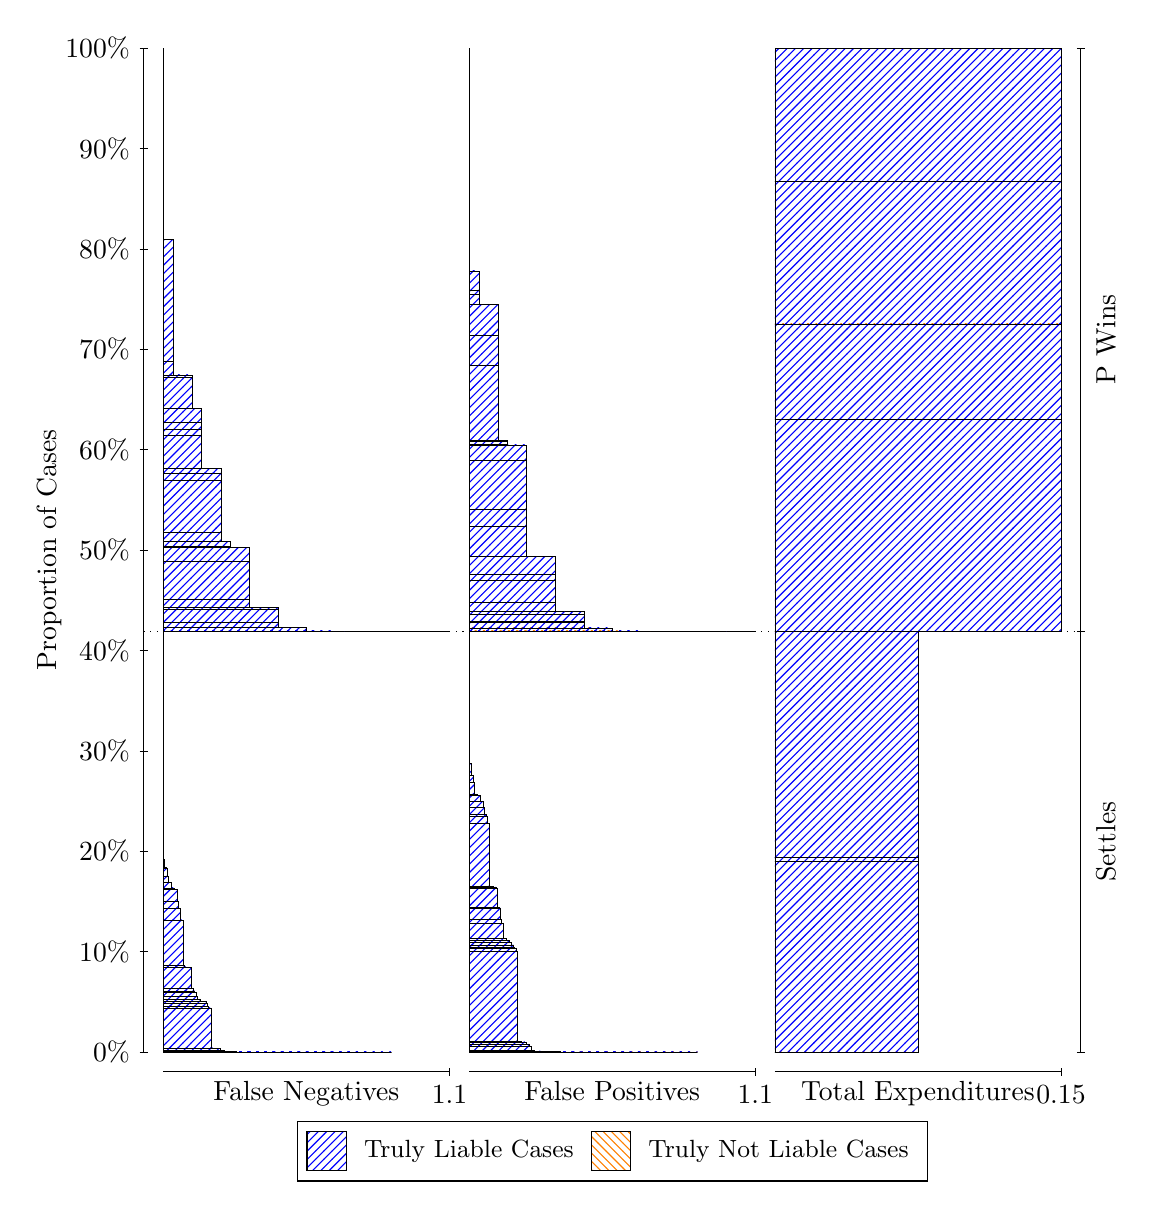
\begin{tikzpicture}
\draw[black, very thin] (1.5,1.75) -- (1.5,14.5);
\node[rotate=90, anchor=center] at (0.3, 8.125) {Proportion of Cases};
\draw[black, very thin] (1.45,1.75) -- (1.55,1.75);
\node[anchor=east] at (1.45, 1.75) {0\%};
\draw[black, very thin] (1.45,3.025) -- (1.55,3.025);
\node[anchor=east] at (1.45, 3.025) {10\%};
\draw[black, very thin] (1.45,4.3) -- (1.55,4.3);
\node[anchor=east] at (1.45, 4.3) {20\%};
\draw[black, very thin] (1.45,5.575) -- (1.55,5.575);
\node[anchor=east] at (1.45, 5.575) {30\%};
\draw[black, very thin] (1.45,6.85) -- (1.55,6.85);
\node[anchor=east] at (1.45, 6.85) {40\%};
\draw[black, very thin] (1.45,8.125) -- (1.55,8.125);
\node[anchor=east] at (1.45, 8.125) {50\%};
\draw[black, very thin] (1.45,9.4) -- (1.55,9.4);
\node[anchor=east] at (1.45, 9.4) {60\%};
\draw[black, very thin] (1.45,10.675) -- (1.55,10.675);
\node[anchor=east] at (1.45, 10.675) {70\%};
\draw[black, very thin] (1.45,11.95) -- (1.55,11.95);
\node[anchor=east] at (1.45, 11.95) {80\%};
\draw[black, very thin] (1.45,13.225) -- (1.55,13.225);
\node[anchor=east] at (1.45, 13.225) {90\%};
\draw[black, very thin] (1.45,14.5) -- (1.55,14.5);
\node[anchor=east] at (1.45, 14.5) {100\%};

\draw[black, very thin] (13.4,1.75) -- (13.4,14.5);
\draw[black, very thin] (13.35,1.75) -- (13.45,1.75);
\node[anchor=west] at (13.35, 1.75) {};
\draw[black, very thin] (13.35,7.0927) -- (13.45,7.0927);
\node[anchor=west] at (13.35, 7.0927) {};
\draw[black, very thin] (13.35,14.5) -- (13.45,14.5);
\node[anchor=west] at (13.35, 14.5) {};

\draw[black, very thin, pattern color=blue, pattern=north east lines] (1.75,1.75) rectangle (4.6485,1.75);
\draw[black, very thin, pattern color=blue, pattern=north east lines] (1.75,1.75) rectangle (4.4852,1.75);
\draw[black, very thin, pattern color=blue, pattern=north east lines] (1.75,1.75) rectangle (4.3219,1.75);
\draw[black, very thin, pattern color=blue, pattern=north east lines] (1.75,1.75) rectangle (4.2856,1.75);
\draw[black, very thin, pattern color=blue, pattern=north east lines] (1.75,1.75) rectangle (4.1586,1.75);
\draw[black, very thin, pattern color=blue, pattern=north east lines] (1.75,1.75) rectangle (4.1223,1.75);
\draw[black, very thin, pattern color=blue, pattern=north east lines] (1.75,1.75) rectangle (3.9953,1.75);
\draw[black, very thin, pattern color=blue, pattern=north east lines] (1.75,1.75) rectangle (3.959,1.75);
\draw[black, very thin, pattern color=blue, pattern=north east lines] (1.75,1.75) rectangle (3.9227,1.75);
\draw[black, very thin, pattern color=blue, pattern=north east lines] (1.75,1.75) rectangle (3.832,1.75);
\draw[black, very thin, pattern color=blue, pattern=north east lines] (1.75,1.75) rectangle (3.7957,1.75);
\draw[black, very thin, pattern color=blue, pattern=north east lines] (1.75,1.75) rectangle (3.7594,1.75);
\draw[black, very thin, pattern color=blue, pattern=north east lines] (1.75,1.75) rectangle (3.6687,1.75);
\draw[black, very thin, pattern color=blue, pattern=north east lines] (1.75,1.75) rectangle (3.6324,1.75);
\draw[black, very thin, pattern color=blue, pattern=north east lines] (1.75,1.75) rectangle (3.5962,1.75);
\draw[black, very thin, pattern color=blue, pattern=north east lines] (1.75,1.75) rectangle (3.5599,1.75);
\draw[black, very thin, pattern color=blue, pattern=north east lines] (1.75,1.75) rectangle (3.5054,1.75);
\draw[black, very thin, pattern color=blue, pattern=north east lines] (1.75,1.75) rectangle (3.4691,1.75);
\draw[black, very thin, pattern color=blue, pattern=north east lines] (1.75,1.75) rectangle (3.4329,1.75);
\draw[black, very thin, pattern color=blue, pattern=north east lines] (1.75,1.75) rectangle (3.3966,1.75);
\draw[black, very thin, pattern color=blue, pattern=north east lines] (1.75,1.75) rectangle (3.3421,1.75);
\draw[black, very thin, pattern color=blue, pattern=north east lines] (1.75,1.75) rectangle (3.3058,1.75);
\draw[black, very thin, pattern color=blue, pattern=north east lines] (1.75,1.75) rectangle (3.2696,1.75);
\draw[black, very thin, pattern color=blue, pattern=north east lines] (1.75,1.75) rectangle (3.2333,1.75);
\draw[black, very thin, pattern color=blue, pattern=north east lines] (1.75,1.75) rectangle (3.197,1.75);
\draw[black, very thin, pattern color=blue, pattern=north east lines] (1.75,1.75) rectangle (3.1788,1.75);
\draw[black, very thin, pattern color=blue, pattern=north east lines] (1.75,1.75) rectangle (3.1426,1.75);
\draw[black, very thin, pattern color=blue, pattern=north east lines] (1.75,1.75) rectangle (3.1063,1.75);
\draw[black, very thin, pattern color=blue, pattern=north east lines] (1.75,1.75) rectangle (3.07,1.75);
\draw[black, very thin, pattern color=blue, pattern=north east lines] (1.75,1.75) rectangle (3.0337,1.75);
\draw[black, very thin, pattern color=blue, pattern=north east lines] (1.75,1.75) rectangle (3.0155,1.75);
\draw[black, very thin, pattern color=blue, pattern=north east lines] (1.75,1.75) rectangle (2.9793,1.75);
\draw[black, very thin, pattern color=blue, pattern=north east lines] (1.75,1.75) rectangle (2.943,1.75);
\draw[black, very thin, pattern color=blue, pattern=north east lines] (1.75,1.75) rectangle (2.9067,1.7501);
\draw[black, very thin, pattern color=blue, pattern=north east lines] (1.75,1.7501) rectangle (2.8704,1.7501);
\draw[black, very thin, pattern color=blue, pattern=north east lines] (1.75,1.7501) rectangle (2.8522,1.7502);
\draw[black, very thin, pattern color=blue, pattern=north east lines] (1.75,1.7502) rectangle (2.8341,1.7507);
\draw[black, very thin, pattern color=blue, pattern=north east lines] (1.75,1.7507) rectangle (2.816,1.7507);
\draw[black, very thin, pattern color=blue, pattern=north east lines] (1.75,1.7507) rectangle (2.7797,1.7507);
\draw[black, very thin, pattern color=blue, pattern=north east lines] (1.75,1.7507) rectangle (2.7434,1.7508);
\draw[black, very thin, pattern color=blue, pattern=north east lines] (1.75,1.7508) rectangle (2.7071,1.7509);
\draw[black, very thin, pattern color=blue, pattern=north east lines] (1.75,1.7509) rectangle (2.689,1.7522);
\draw[black, very thin, pattern color=blue, pattern=north east lines] (1.75,1.7522) rectangle (2.6708,1.7542);
\draw[black, very thin, pattern color=blue, pattern=north east lines] (1.75,1.7542) rectangle (2.6527,1.7547);
\draw[black, very thin, pattern color=blue, pattern=north east lines] (1.75,1.7547) rectangle (2.6164,1.7548);
\draw[black, very thin, pattern color=blue, pattern=north east lines] (1.75,1.7548) rectangle (2.5801,1.7566);
\draw[black, very thin, pattern color=blue, pattern=north east lines] (1.75,1.7566) rectangle (2.5438,1.7585);
\draw[black, very thin, pattern color=blue, pattern=north east lines] (1.75,1.7585) rectangle (2.5257,1.7684);
\draw[black, very thin, pattern color=blue, pattern=north east lines] (1.75,1.7684) rectangle (2.5075,1.7715);
\draw[black, very thin, pattern color=blue, pattern=north east lines] (1.75,1.7715) rectangle (2.4894,1.7737);
\draw[black, very thin, pattern color=blue, pattern=north east lines] (1.75,1.7737) rectangle (2.4712,1.7998);
\draw[black, very thin, pattern color=blue, pattern=north east lines] (1.75,1.7998) rectangle (2.4531,1.7999);
\draw[black, very thin, pattern color=blue, pattern=north east lines] (1.75,1.7999) rectangle (2.4168,1.8001);
\draw[black, very thin, pattern color=blue, pattern=north east lines] (1.75,1.8001) rectangle (2.3805,1.8031);
\draw[black, very thin, pattern color=blue, pattern=north east lines] (1.75,1.8031) rectangle (2.3624,2.3067);
\draw[black, very thin, pattern color=blue, pattern=north east lines] (1.75,2.3067) rectangle (2.3442,2.3086);
\draw[black, very thin, pattern color=blue, pattern=north east lines] (1.75,2.3086) rectangle (2.3261,2.3357);
\draw[black, very thin, pattern color=blue, pattern=north east lines] (1.75,2.3357) rectangle (2.3079,2.3682);
\draw[black, very thin, pattern color=blue, pattern=north east lines] (1.75,2.3682) rectangle (2.2898,2.3891);
\draw[black, very thin, pattern color=blue, pattern=north east lines] (1.75,2.3891) rectangle (2.2535,2.3921);
\draw[black, very thin, pattern color=blue, pattern=north east lines] (1.75,2.3921) rectangle (2.2172,2.4217);
\draw[black, very thin, pattern color=blue, pattern=north east lines] (1.75,2.4217) rectangle (2.1809,2.4513);
\draw[black, very thin, pattern color=blue, pattern=north east lines] (1.75,2.4513) rectangle (2.1628,2.5067);
\draw[black, very thin, pattern color=blue, pattern=north east lines] (1.75,2.5067) rectangle (2.1446,2.5272);
\draw[black, very thin, pattern color=blue, pattern=north east lines] (1.75,2.5272) rectangle (2.1265,2.5601);
\draw[black, very thin, pattern color=blue, pattern=north east lines] (1.75,2.5601) rectangle (2.1083,2.8276);
\draw[black, very thin, pattern color=blue, pattern=north east lines] (1.75,2.8276) rectangle (2.0902,2.8295);
\draw[black, very thin, pattern color=blue, pattern=north east lines] (1.75,2.8295) rectangle (2.0539,2.8313);
\draw[black, very thin, pattern color=blue, pattern=north east lines] (1.75,2.8313) rectangle (2.0176,2.8505);
\draw[black, very thin, pattern color=blue, pattern=north east lines] (1.75,2.8505) rectangle (1.9995,3.4218);
\draw[black, very thin, pattern color=blue, pattern=north east lines] (1.75,3.4218) rectangle (1.9813,3.4269);
\draw[black, very thin, pattern color=blue, pattern=north east lines] (1.75,3.4269) rectangle (1.9632,3.5724);
\draw[black, very thin, pattern color=blue, pattern=north east lines] (1.75,3.5724) rectangle (1.945,3.6667);
\draw[black, very thin, pattern color=blue, pattern=north east lines] (1.75,3.6667) rectangle (1.9269,3.8149);
\draw[black, very thin, pattern color=blue, pattern=north east lines] (1.75,3.8149) rectangle (1.8906,3.834);
\draw[black, very thin, pattern color=blue, pattern=north east lines] (1.75,3.834) rectangle (1.8543,3.9086);
\draw[black, very thin, pattern color=blue, pattern=north east lines] (1.75,3.9086) rectangle (1.818,3.9831);
\draw[black, very thin, pattern color=blue, pattern=north east lines] (1.75,3.9831) rectangle (1.7999,4.0775);
\draw[black, very thin, pattern color=blue, pattern=north east lines] (1.75,4.0775) rectangle (1.7818,4.1011);
\draw[black, very thin, pattern color=blue, pattern=north east lines] (1.75,4.1011) rectangle (1.7636,4.1943);
\draw[black, very thin, pattern color=orange, pattern=north west lines] (1.75,4.1943) rectangle (1.75,4.1943);
\draw[black, very thin, pattern color=blue, pattern=north east lines] (1.75,4.1943) rectangle (1.75,7.0927);
\draw[black, very thin, pattern color=blue, pattern=north east lines] (1.75,7.0927) rectangle (5.3833,7.0927);
\draw[black, very thin, pattern color=blue, pattern=north east lines] (1.75,7.0927) rectangle (5.0205,7.0927);
\draw[black, very thin, pattern color=blue, pattern=north east lines] (1.75,7.0927) rectangle (4.6576,7.0927);
\draw[black, very thin, pattern color=blue, pattern=north east lines] (1.75,7.0927) rectangle (4.4126,7.0927);
\draw[black, very thin, pattern color=blue, pattern=north east lines] (1.75,7.0927) rectangle (4.2947,7.0929);
\draw[black, very thin, pattern color=blue, pattern=north east lines] (1.75,7.0929) rectangle (4.2947,7.0931);
\draw[black, very thin, pattern color=blue, pattern=north east lines] (1.75,7.0931) rectangle (4.0498,7.0931);
\draw[black, very thin, pattern color=blue, pattern=north east lines] (1.75,7.0931) rectangle (3.9318,7.0967);
\draw[black, very thin, pattern color=blue, pattern=north east lines] (1.75,7.0967) rectangle (3.9318,7.0986);
\draw[black, very thin, pattern color=blue, pattern=north east lines] (1.75,7.0986) rectangle (3.6869,7.0986);
\draw[black, very thin, pattern color=blue, pattern=north east lines] (1.75,7.0986) rectangle (3.6869,7.0986);
\draw[black, very thin, pattern color=blue, pattern=north east lines] (1.75,7.0986) rectangle (3.5689,7.1457);
\draw[black, very thin, pattern color=blue, pattern=north east lines] (1.75,7.1457) rectangle (3.324,7.1457);
\draw[black, very thin, pattern color=blue, pattern=north east lines] (1.75,7.1457) rectangle (3.324,7.1457);
\draw[black, very thin, pattern color=blue, pattern=north east lines] (1.75,7.1457) rectangle (3.2061,7.2105);
\draw[black, very thin, pattern color=blue, pattern=north east lines] (1.75,7.2105) rectangle (3.2061,7.3681);
\draw[black, very thin, pattern color=blue, pattern=north east lines] (1.75,7.3681) rectangle (3.2061,7.3956);
\draw[black, very thin, pattern color=blue, pattern=north east lines] (1.75,7.3956) rectangle (2.9611,7.3969);
\draw[black, very thin, pattern color=blue, pattern=north east lines] (1.75,7.3969) rectangle (2.9611,7.3972);
\draw[black, very thin, pattern color=blue, pattern=north east lines] (1.75,7.3972) rectangle (2.9611,7.3976);
\draw[black, very thin, pattern color=blue, pattern=north east lines] (1.75,7.3976) rectangle (2.8432,7.4933);
\draw[black, very thin, pattern color=blue, pattern=north east lines] (1.75,7.4933) rectangle (2.8432,7.9787);
\draw[black, very thin, pattern color=blue, pattern=north east lines] (1.75,7.9787) rectangle (2.8432,8.1604);
\draw[black, very thin, pattern color=blue, pattern=north east lines] (1.75,8.1604) rectangle (2.5982,8.1699);
\draw[black, very thin, pattern color=blue, pattern=north east lines] (1.75,8.1699) rectangle (2.5982,8.2322);
\draw[black, very thin, pattern color=blue, pattern=north east lines] (1.75,8.2322) rectangle (2.4803,8.3496);
\draw[black, very thin, pattern color=blue, pattern=north east lines] (1.75,8.3496) rectangle (2.4803,9.0133);
\draw[black, very thin, pattern color=blue, pattern=north east lines] (1.75,9.0133) rectangle (2.4803,9.1055);
\draw[black, very thin, pattern color=blue, pattern=north east lines] (1.75,9.1055) rectangle (2.4803,9.1609);
\draw[black, very thin, pattern color=blue, pattern=north east lines] (1.75,9.1609) rectangle (2.2354,9.5806);
\draw[black, very thin, pattern color=blue, pattern=north east lines] (1.75,9.5806) rectangle (2.2354,9.6587);
\draw[black, very thin, pattern color=blue, pattern=north east lines] (1.75,9.6587) rectangle (2.2354,9.7412);
\draw[black, very thin, pattern color=blue, pattern=north east lines] (1.75,9.7412) rectangle (2.2354,9.9241);
\draw[black, very thin, pattern color=blue, pattern=north east lines] (1.75,9.9241) rectangle (2.1174,10.317);
\draw[black, very thin, pattern color=blue, pattern=north east lines] (1.75,10.317) rectangle (2.1174,10.349);
\draw[black, very thin, pattern color=blue, pattern=north east lines] (1.75,10.349) rectangle (1.8725,10.516);
\draw[black, very thin, pattern color=blue, pattern=north east lines] (1.75,10.516) rectangle (1.8725,12.071);
\draw[black, very thin, pattern color=blue, pattern=north east lines] (1.75,12.071) rectangle (1.7545,12.131);
\draw[black, very thin, pattern color=blue, pattern=north east lines] (1.75,12.131) rectangle (1.7545,12.132);
\draw[black, very thin, pattern color=blue, pattern=north east lines] (1.75,12.132) rectangle (1.7545,12.132);
\draw[black, very thin, pattern color=orange, pattern=north west lines] (1.75,12.132) rectangle (1.75,12.132);
\draw[black, very thin, pattern color=blue, pattern=north east lines] (1.75,12.132) rectangle (1.75,14.5);
\draw[black, very thin, pattern color=orange, pattern=north west lines] (5.6333,1.75) rectangle (8.5318,1.75);
\draw[black, very thin, pattern color=blue, pattern=north east lines] (5.6333,1.75) rectangle (8.5318,1.75);
\draw[black, very thin, pattern color=orange, pattern=north west lines] (5.6333,1.75) rectangle (8.3685,1.75);
\draw[black, very thin, pattern color=blue, pattern=north east lines] (5.6333,1.75) rectangle (8.3685,1.75);
\draw[black, very thin, pattern color=orange, pattern=north west lines] (5.6333,1.75) rectangle (8.2052,1.75);
\draw[black, very thin, pattern color=blue, pattern=north east lines] (5.6333,1.75) rectangle (8.2052,1.75);
\draw[black, very thin, pattern color=blue, pattern=north east lines] (5.6333,1.75) rectangle (8.169,1.75);
\draw[black, very thin, pattern color=orange, pattern=north west lines] (5.6333,1.75) rectangle (8.0419,1.75);
\draw[black, very thin, pattern color=blue, pattern=north east lines] (5.6333,1.75) rectangle (8.0419,1.75);
\draw[black, very thin, pattern color=blue, pattern=north east lines] (5.6333,1.75) rectangle (8.0057,1.75);
\draw[black, very thin, pattern color=orange, pattern=north west lines] (5.6333,1.75) rectangle (7.8787,1.75);
\draw[black, very thin, pattern color=blue, pattern=north east lines] (5.6333,1.75) rectangle (7.8787,1.75);
\draw[black, very thin, pattern color=blue, pattern=north east lines] (5.6333,1.75) rectangle (7.8424,1.75);
\draw[black, very thin, pattern color=blue, pattern=north east lines] (5.6333,1.75) rectangle (7.8061,1.75);
\draw[black, very thin, pattern color=orange, pattern=north west lines] (5.6333,1.75) rectangle (7.7154,1.75);
\draw[black, very thin, pattern color=blue, pattern=north east lines] (5.6333,1.75) rectangle (7.7154,1.75);
\draw[black, very thin, pattern color=blue, pattern=north east lines] (5.6333,1.75) rectangle (7.6791,1.75);
\draw[black, very thin, pattern color=blue, pattern=north east lines] (5.6333,1.75) rectangle (7.6428,1.75);
\draw[black, very thin, pattern color=orange, pattern=north west lines] (5.6333,1.75) rectangle (7.5521,1.75);
\draw[black, very thin, pattern color=blue, pattern=north east lines] (5.6333,1.75) rectangle (7.5521,1.75);
\draw[black, very thin, pattern color=blue, pattern=north east lines] (5.6333,1.75) rectangle (7.5158,1.75);
\draw[black, very thin, pattern color=blue, pattern=north east lines] (5.6333,1.75) rectangle (7.4795,1.75);
\draw[black, very thin, pattern color=blue, pattern=north east lines] (5.6333,1.75) rectangle (7.4432,1.75);
\draw[black, very thin, pattern color=orange, pattern=north west lines] (5.6333,1.75) rectangle (7.3888,1.75);
\draw[black, very thin, pattern color=blue, pattern=north east lines] (5.6333,1.75) rectangle (7.3888,1.75);
\draw[black, very thin, pattern color=blue, pattern=north east lines] (5.6333,1.75) rectangle (7.3525,1.75);
\draw[black, very thin, pattern color=blue, pattern=north east lines] (5.6333,1.75) rectangle (7.3162,1.75);
\draw[black, very thin, pattern color=blue, pattern=north east lines] (5.6333,1.75) rectangle (7.2799,1.75);
\draw[black, very thin, pattern color=orange, pattern=north west lines] (5.6333,1.75) rectangle (7.2255,1.75);
\draw[black, very thin, pattern color=blue, pattern=north east lines] (5.6333,1.75) rectangle (7.2255,1.75);
\draw[black, very thin, pattern color=blue, pattern=north east lines] (5.6333,1.75) rectangle (7.1892,1.75);
\draw[black, very thin, pattern color=blue, pattern=north east lines] (5.6333,1.75) rectangle (7.1529,1.75);
\draw[black, very thin, pattern color=blue, pattern=north east lines] (5.6333,1.75) rectangle (7.1166,1.75);
\draw[black, very thin, pattern color=blue, pattern=north east lines] (5.6333,1.75) rectangle (7.0803,1.75);
\draw[black, very thin, pattern color=orange, pattern=north west lines] (5.6333,1.75) rectangle (7.0622,1.75);
\draw[black, very thin, pattern color=blue, pattern=north east lines] (5.6333,1.75) rectangle (7.0622,1.75);
\draw[black, very thin, pattern color=blue, pattern=north east lines] (5.6333,1.75) rectangle (7.0259,1.75);
\draw[black, very thin, pattern color=blue, pattern=north east lines] (5.6333,1.75) rectangle (6.9896,1.75);
\draw[black, very thin, pattern color=blue, pattern=north east lines] (5.6333,1.75) rectangle (6.9533,1.7501);
\draw[black, very thin, pattern color=blue, pattern=north east lines] (5.6333,1.7501) rectangle (6.917,1.7501);
\draw[black, very thin, pattern color=orange, pattern=north west lines] (5.6333,1.7501) rectangle (6.8989,1.7501);
\draw[black, very thin, pattern color=blue, pattern=north east lines] (5.6333,1.7501) rectangle (6.8989,1.7502);
\draw[black, very thin, pattern color=blue, pattern=north east lines] (5.6333,1.7502) rectangle (6.8626,1.7502);
\draw[black, very thin, pattern color=blue, pattern=north east lines] (5.6333,1.7502) rectangle (6.8263,1.7503);
\draw[black, very thin, pattern color=blue, pattern=north east lines] (5.6333,1.7503) rectangle (6.79,1.7526);
\draw[black, very thin, pattern color=blue, pattern=north east lines] (5.6333,1.7526) rectangle (6.7537,1.7532);
\draw[black, very thin, pattern color=orange, pattern=north west lines] (5.6333,1.7532) rectangle (6.7356,1.7532);
\draw[black, very thin, pattern color=blue, pattern=north east lines] (5.6333,1.7532) rectangle (6.7356,1.7532);
\draw[black, very thin, pattern color=blue, pattern=north east lines] (5.6333,1.7532) rectangle (6.7174,1.7538);
\draw[black, very thin, pattern color=blue, pattern=north east lines] (5.6333,1.7538) rectangle (6.6993,1.7538);
\draw[black, very thin, pattern color=blue, pattern=north east lines] (5.6333,1.7538) rectangle (6.663,1.7539);
\draw[black, very thin, pattern color=blue, pattern=north east lines] (5.6333,1.7539) rectangle (6.6267,1.7541);
\draw[black, very thin, pattern color=blue, pattern=north east lines] (5.6333,1.7541) rectangle (6.5904,1.7588);
\draw[black, very thin, pattern color=orange, pattern=north west lines] (5.6333,1.7588) rectangle (6.5723,1.7588);
\draw[black, very thin, pattern color=blue, pattern=north east lines] (5.6333,1.7588) rectangle (6.5723,1.7592);
\draw[black, very thin, pattern color=blue, pattern=north east lines] (5.6333,1.7592) rectangle (6.5541,1.7611);
\draw[black, very thin, pattern color=blue, pattern=north east lines] (5.6333,1.7611) rectangle (6.536,1.7632);
\draw[black, very thin, pattern color=blue, pattern=north east lines] (5.6333,1.7632) rectangle (6.4997,1.7651);
\draw[black, very thin, pattern color=blue, pattern=north east lines] (5.6333,1.7651) rectangle (6.4634,1.7681);
\draw[black, very thin, pattern color=blue, pattern=north east lines] (5.6333,1.7681) rectangle (6.4271,1.8164);
\draw[black, very thin, pattern color=orange, pattern=north west lines] (5.6333,1.8164) rectangle (6.409,1.8164);
\draw[black, very thin, pattern color=blue, pattern=north east lines] (5.6333,1.8164) rectangle (6.409,1.8264);
\draw[black, very thin, pattern color=blue, pattern=north east lines] (5.6333,1.8264) rectangle (6.3908,1.85);
\draw[black, very thin, pattern color=blue, pattern=north east lines] (5.6333,1.85) rectangle (6.3727,1.8502);
\draw[black, very thin, pattern color=blue, pattern=north east lines] (5.6333,1.8502) rectangle (6.3546,1.8759);
\draw[black, very thin, pattern color=blue, pattern=north east lines] (5.6333,1.8759) rectangle (6.3364,1.8789);
\draw[black, very thin, pattern color=blue, pattern=north east lines] (5.6333,1.8789) rectangle (6.3001,1.8808);
\draw[black, very thin, pattern color=blue, pattern=north east lines] (5.6333,1.8808) rectangle (6.2638,1.8826);
\draw[black, very thin, pattern color=orange, pattern=north west lines] (5.6333,1.8826) rectangle (6.2457,1.8826);
\draw[black, very thin, pattern color=blue, pattern=north east lines] (5.6333,1.8826) rectangle (6.2457,3.0241);
\draw[black, very thin, pattern color=blue, pattern=north east lines] (5.6333,3.0241) rectangle (6.2275,3.0724);
\draw[black, very thin, pattern color=blue, pattern=north east lines] (5.6333,3.0724) rectangle (6.2094,3.0778);
\draw[black, very thin, pattern color=blue, pattern=north east lines] (5.6333,3.0778) rectangle (6.1913,3.1103);
\draw[black, very thin, pattern color=blue, pattern=north east lines] (5.6333,3.1103) rectangle (6.1731,3.1403);
\draw[black, very thin, pattern color=blue, pattern=north east lines] (5.6333,3.1403) rectangle (6.1368,3.1699);
\draw[black, very thin, pattern color=blue, pattern=north east lines] (5.6333,3.1699) rectangle (6.1005,3.1891);
\draw[black, very thin, pattern color=blue, pattern=north east lines] (5.6333,3.1891) rectangle (6.0643,3.382);
\draw[black, very thin, pattern color=blue, pattern=north east lines] (5.6333,3.382) rectangle (6.0461,3.4375);
\draw[black, very thin, pattern color=blue, pattern=north east lines] (5.6333,3.4375) rectangle (6.028,3.5812);
\draw[black, very thin, pattern color=blue, pattern=north east lines] (5.6333,3.5812) rectangle (6.0098,3.5835);
\draw[black, very thin, pattern color=blue, pattern=north east lines] (5.6333,3.5835) rectangle (5.9917,3.8274);
\draw[black, very thin, pattern color=blue, pattern=north east lines] (5.6333,3.8274) rectangle (5.9735,3.8465);
\draw[black, very thin, pattern color=blue, pattern=north east lines] (5.6333,3.8465) rectangle (5.9372,3.8512);
\draw[black, very thin, pattern color=blue, pattern=north east lines] (5.6333,3.8512) rectangle (5.901,3.856);
\draw[black, very thin, pattern color=blue, pattern=north east lines] (5.6333,3.856) rectangle (5.8828,4.6483);
\draw[black, very thin, pattern color=blue, pattern=north east lines] (5.6333,4.6483) rectangle (5.8647,4.7415);
\draw[black, very thin, pattern color=blue, pattern=north east lines] (5.6333,4.7415) rectangle (5.8465,4.7652);
\draw[black, very thin, pattern color=blue, pattern=north east lines] (5.6333,4.7652) rectangle (5.8284,4.8595);
\draw[black, very thin, pattern color=blue, pattern=north east lines] (5.6333,4.8595) rectangle (5.8102,4.9341);
\draw[black, very thin, pattern color=blue, pattern=north east lines] (5.6333,4.9341) rectangle (5.7739,5.0086);
\draw[black, very thin, pattern color=blue, pattern=north east lines] (5.6333,5.0086) rectangle (5.7377,5.0278);
\draw[black, very thin, pattern color=blue, pattern=north east lines] (5.6333,5.0278) rectangle (5.7014,5.1759);
\draw[black, very thin, pattern color=blue, pattern=north east lines] (5.6333,5.1759) rectangle (5.6832,5.2703);
\draw[black, very thin, pattern color=blue, pattern=north east lines] (5.6333,5.2703) rectangle (5.6651,5.4158);
\draw[black, very thin, pattern color=blue, pattern=north east lines] (5.6333,5.4158) rectangle (5.6469,5.4209);
\draw[black, very thin, pattern color=blue, pattern=north east lines] (5.6333,5.4209) rectangle (5.6333,7.0927);
\draw[black, very thin, pattern color=orange, pattern=north west lines] (5.6333,7.0927) rectangle (9.2667,7.0927);
\draw[black, very thin, pattern color=blue, pattern=north east lines] (5.6333,7.0927) rectangle (9.2667,7.0927);
\draw[black, very thin, pattern color=orange, pattern=north west lines] (5.6333,7.0927) rectangle (8.9038,7.0927);
\draw[black, very thin, pattern color=blue, pattern=north east lines] (5.6333,7.0927) rectangle (8.9038,7.0927);
\draw[black, very thin, pattern color=blue, pattern=north east lines] (5.6333,7.0927) rectangle (8.5409,7.0927);
\draw[black, very thin, pattern color=orange, pattern=north west lines] (5.6333,7.0927) rectangle (8.5409,7.0927);
\draw[black, very thin, pattern color=blue, pattern=north east lines] (5.6333,7.0927) rectangle (8.5409,7.0927);
\draw[black, very thin, pattern color=orange, pattern=north west lines] (5.6333,7.0927) rectangle (8.296,7.0927);
\draw[black, very thin, pattern color=blue, pattern=north east lines] (5.6333,7.0927) rectangle (8.296,7.0927);
\draw[black, very thin, pattern color=blue, pattern=north east lines] (5.6333,7.0927) rectangle (8.178,7.0928);
\draw[black, very thin, pattern color=blue, pattern=north east lines] (5.6333,7.0928) rectangle (8.178,7.0929);
\draw[black, very thin, pattern color=orange, pattern=north west lines] (5.6333,7.0929) rectangle (8.178,7.0929);
\draw[black, very thin, pattern color=blue, pattern=north east lines] (5.6333,7.0929) rectangle (8.178,7.093);
\draw[black, very thin, pattern color=orange, pattern=north west lines] (5.6333,7.093) rectangle (7.9331,7.093);
\draw[black, very thin, pattern color=blue, pattern=north east lines] (5.6333,7.093) rectangle (7.9331,7.093);
\draw[black, very thin, pattern color=orange, pattern=north west lines] (5.6333,7.093) rectangle (7.8151,7.093);
\draw[black, very thin, pattern color=blue, pattern=north east lines] (5.6333,7.093) rectangle (7.8151,7.0958);
\draw[black, very thin, pattern color=blue, pattern=north east lines] (5.6333,7.0958) rectangle (7.8151,7.0969);
\draw[black, very thin, pattern color=blue, pattern=north east lines] (5.6333,7.0969) rectangle (7.8151,7.0976);
\draw[black, very thin, pattern color=orange, pattern=north west lines] (5.6333,7.0976) rectangle (7.5702,7.0976);
\draw[black, very thin, pattern color=blue, pattern=north east lines] (5.6333,7.0976) rectangle (7.5702,7.0976);
\draw[black, very thin, pattern color=blue, pattern=north east lines] (5.6333,7.0976) rectangle (7.5702,7.0976);
\draw[black, very thin, pattern color=orange, pattern=north west lines] (5.6333,7.0976) rectangle (7.4523,7.0976);
\draw[black, very thin, pattern color=blue, pattern=north east lines] (5.6333,7.0976) rectangle (7.4523,7.1295);
\draw[black, very thin, pattern color=blue, pattern=north east lines] (5.6333,7.1295) rectangle (7.4523,7.1371);
\draw[black, very thin, pattern color=blue, pattern=north east lines] (5.6333,7.1371) rectangle (7.2073,7.1371);
\draw[black, very thin, pattern color=orange, pattern=north west lines] (5.6333,7.1371) rectangle (7.2073,7.1371);
\draw[black, very thin, pattern color=blue, pattern=north east lines] (5.6333,7.1371) rectangle (7.2073,7.1371);
\draw[black, very thin, pattern color=blue, pattern=north east lines] (5.6333,7.1371) rectangle (7.0894,7.2027);
\draw[black, very thin, pattern color=blue, pattern=north east lines] (5.6333,7.2027) rectangle (7.0894,7.2217);
\draw[black, very thin, pattern color=orange, pattern=north west lines] (5.6333,7.2217) rectangle (7.0894,7.2217);
\draw[black, very thin, pattern color=blue, pattern=north east lines] (5.6333,7.2217) rectangle (7.0894,7.3056);
\draw[black, very thin, pattern color=blue, pattern=north east lines] (5.6333,7.3056) rectangle (7.0894,7.3463);
\draw[black, very thin, pattern color=blue, pattern=north east lines] (5.6333,7.3463) rectangle (6.8444,7.3463);
\draw[black, very thin, pattern color=orange, pattern=north west lines] (5.6333,7.3463) rectangle (6.8444,7.3463);
\draw[black, very thin, pattern color=blue, pattern=north east lines] (5.6333,7.3463) rectangle (6.8444,7.3463);
\draw[black, very thin, pattern color=blue, pattern=north east lines] (5.6333,7.3463) rectangle (6.7265,7.4649);
\draw[black, very thin, pattern color=blue, pattern=north east lines] (5.6333,7.4649) rectangle (6.7265,7.7423);
\draw[black, very thin, pattern color=orange, pattern=north west lines] (5.6333,7.7423) rectangle (6.7265,7.7423);
\draw[black, very thin, pattern color=blue, pattern=north east lines] (5.6333,7.7423) rectangle (6.7265,7.8189);
\draw[black, very thin, pattern color=blue, pattern=north east lines] (5.6333,7.8189) rectangle (6.7265,8.0423);
\draw[black, very thin, pattern color=blue, pattern=north east lines] (5.6333,8.0423) rectangle (6.4816,8.0423);
\draw[black, very thin, pattern color=orange, pattern=north west lines] (5.6333,8.0423) rectangle (6.4816,8.0423);
\draw[black, very thin, pattern color=blue, pattern=north east lines] (5.6333,8.0423) rectangle (6.4816,8.0427);
\draw[black, very thin, pattern color=blue, pattern=north east lines] (5.6333,8.0427) rectangle (6.3636,8.4213);
\draw[black, very thin, pattern color=blue, pattern=north east lines] (5.6333,8.4213) rectangle (6.3636,8.6418);
\draw[black, very thin, pattern color=blue, pattern=north east lines] (5.6333,8.6418) rectangle (6.3636,9.2618);
\draw[black, very thin, pattern color=blue, pattern=north east lines] (5.6333,9.2618) rectangle (6.3636,9.4606);
\draw[black, very thin, pattern color=blue, pattern=north east lines] (5.6333,9.4606) rectangle (6.1187,9.4619);
\draw[black, very thin, pattern color=orange, pattern=north west lines] (5.6333,9.4619) rectangle (6.1187,9.4619);
\draw[black, very thin, pattern color=blue, pattern=north east lines] (5.6333,9.4619) rectangle (6.1187,9.503);
\draw[black, very thin, pattern color=blue, pattern=north east lines] (5.6333,9.503) rectangle (6.1187,9.5206);
\draw[black, very thin, pattern color=blue, pattern=north east lines] (5.6333,9.5206) rectangle (6.1187,9.5217);
\draw[black, very thin, pattern color=blue, pattern=north east lines] (5.6333,9.5217) rectangle (6.0007,10.471);
\draw[black, very thin, pattern color=blue, pattern=north east lines] (5.6333,10.471) rectangle (6.0007,10.856);
\draw[black, very thin, pattern color=blue, pattern=north east lines] (5.6333,10.856) rectangle (6.0007,11.244);
\draw[black, very thin, pattern color=blue, pattern=north east lines] (5.6333,11.244) rectangle (5.7558,11.374);
\draw[black, very thin, pattern color=orange, pattern=north west lines] (5.6333,11.374) rectangle (5.7558,11.374);
\draw[black, very thin, pattern color=blue, pattern=north east lines] (5.6333,11.374) rectangle (5.7558,11.425);
\draw[black, very thin, pattern color=blue, pattern=north east lines] (5.6333,11.425) rectangle (5.7558,11.669);
\draw[black, very thin, pattern color=blue, pattern=north east lines] (5.6333,11.669) rectangle (5.6379,11.752);
\draw[black, very thin, pattern color=blue, pattern=north east lines] (5.6333,11.752) rectangle (5.6379,12.349);
\draw[black, very thin, pattern color=blue, pattern=north east lines] (5.6333,12.349) rectangle (5.6379,12.432);
\draw[black, very thin, pattern color=blue, pattern=north east lines] (5.6333,12.432) rectangle (5.6333,14.5);
\draw[black, very thin, pattern color=orange, pattern=north west lines] (9.5167,1.75) rectangle (11.333,1.75);
\draw[black, very thin, pattern color=blue, pattern=north east lines] (9.5167,1.75) rectangle (11.333,4.1722);
\draw[black, very thin, pattern color=orange, pattern=north west lines] (9.5167,4.1722) rectangle (11.333,4.1722);
\draw[black, very thin, pattern color=blue, pattern=north east lines] (9.5167,4.1722) rectangle (11.333,4.2253);
\draw[black, very thin, pattern color=orange, pattern=north west lines] (9.5167,4.2253) rectangle (11.333,4.2253);
\draw[black, very thin, pattern color=blue, pattern=north east lines] (9.5167,4.2253) rectangle (11.333,7.0927);
\draw[black, very thin, pattern color=orange, pattern=north west lines] (9.5167,7.0927) rectangle (13.15,7.0927);
\draw[black, very thin, pattern color=blue, pattern=north east lines] (9.5167,7.0927) rectangle (13.15,9.7875);
\draw[black, very thin, pattern color=orange, pattern=north west lines] (9.5167,9.7875) rectangle (13.15,9.7875);
\draw[black, very thin, pattern color=blue, pattern=north east lines] (9.5167,9.7875) rectangle (13.15,10.997);
\draw[black, very thin, pattern color=orange, pattern=north west lines] (9.5167,10.997) rectangle (13.15,10.997);
\draw[black, very thin, pattern color=blue, pattern=north east lines] (9.5167,10.997) rectangle (13.15,12.803);
\draw[black, very thin, pattern color=orange, pattern=north west lines] (9.5167,12.803) rectangle (13.15,12.803);
\draw[black, very thin, pattern color=blue, pattern=north east lines] (9.5167,12.803) rectangle (13.15,14.5);
\draw[black, dotted] (1.5,7.0927) -- (13.4,7.0927);
\draw[black, very thin] (1.75,1.5) -- (5.3833,1.5);
\node[anchor=north] at (3.5667, 1.5) {False Negatives};
\draw[black, very thin] (5.3833,1.45) -- (5.3833,1.55);
\node[anchor=north] at (5.3833, 1.45) {1.1};

\draw[black, very thin] (5.6333,1.5) -- (9.2667,1.5);
\node[anchor=north] at (7.45, 1.5) {False Positives};
\draw[black, very thin] (9.2667,1.45) -- (9.2667,1.55);
\node[anchor=north] at (9.2667, 1.45) {1.1};

\draw[black, very thin] (9.5167,1.5) -- (13.15,1.5);
\node[anchor=north] at (11.333, 1.5) {Total Expenditures};
\draw[black, very thin] (13.15,1.45) -- (13.15,1.55);
\node[anchor=north] at (13.15, 1.45) {0.15};

\node[black, centered, rotate=90] at (13.72, 4.4213) {Settles};
\node[black, centered, rotate=90] at (13.72, 10.796) {P Wins};

\draw (7.449999999999999,1.5) node[draw=none] (baseCoordinate) {};
\begin{scope}[align=center]
        \matrix[scale=0.5, draw=black, below=0.5cm of baseCoordinate, nodes={draw}, column sep=0.1cm]{
            \node[rectangle, draw, minimum width=0.5cm, minimum height=0.5cm, pattern=north east lines, pattern color=blue] {}; &
            \node[draw=none, font=\small] (B) {Truly Liable Cases}; &
            \node[rectangle, draw, minimum width=0.5cm, minimum height=0.5cm, pattern=north west lines, pattern color=orange] {}; &
            \node[draw=none, font=\small] (B) {Truly Not Liable Cases}; \\
            };
\end{scope}

\end{tikzpicture}
\end{document}